% SGA 3，第 X 篇，第 1 轮英文重建本的中文译本。
% 范围：标题及第 1--3 节，至推论 3.9。
% 依据：Polo--Gille Expo10-8nov09.pdf，原文件第 1--11 页
% （合并阅读版第 679--689 页；印刷页码 63--73，页边页码 77--92）。
% OCR 与 Reinhold 的英文 Markdown 仅用作对比见证。

\setcounter{footnote}{0}
\SGARefTarget{sga3:x:chapter:x}\chapter*{第 X 篇\\
乘法型群的刻画与分类}
\addcontentsline{toc}{chapter}{第 X 篇. 乘法型群的刻画与分类}
\markboth{第 X 篇．乘法型群}
  {第 X 篇．乘法型群}

\begin{center}
  \textit{A. Grothendieck 著}
\end{center}
\begin{NoHyper}
\footnotetext{2009 年 11 月 6 日 xy 版本：增补置于\SGARefLink{sga3:x:section:9}{第~9 节}；已审阅至 \SGARefLink{sga3:x:theorem:8-8}{8.8}。}
\end{NoHyper}

\SGARefTarget{sga3:x:section:1}\section*{1. 等平凡群的分类：基为域的情形}
\addcontentsline{toc}{section}{1. 等平凡群的分类：基为域的情形}

回顾（\SGARefLink{sga3:ix:definition:1:1}{IX~1.1}），若存在有限平展满射态射
\(S'\to S\)，使 \(H'=H\times_S S'\) 可对角化，则称预概形 \(S\) 上的乘法型群
\(H\) 为\emph{等平凡}的。当 \(S\) 连通时，\(S'\) 分解为有限个连通分量
\(S'_i\) 的不交和；因而将 \(S'\) 换成某个 \(S'_i\) 后，可以假定 \(S'\) 连通。
最后，可以找到支配 \(S'\) 的连通有限平展 \(S'_1\)，并使之为 Galois 的，即
\(S\) 上的主齐性丛，其群为 \(\Gamma_S\)，其中 \(\Gamma\) 是通常的有限群
（\(S\) 局部 Noether 时，参见\ SGA~1，V，第~7 和~3 目；一般情形见
EGA~IV\textsubscript{4}，18.2.9）。\footnote{编者注：更准确地说，这由“Galois 理论的公理条件”推出，
参见\ SGA~1，V，第~4~g) 目；当 \(S\) 局部 Noether 时，这些公理已在\emph{同处}
第~7 和~3 目中验证，特别是 \SGARefLink{sga3:x:theorem:3:7}{3.7}，其依据是
SGA~1，I，10.9。后一个结果在 EGA~IV\textsubscript{4}，18.2.9 中不作 Noether 假设得到证明。}
假定如此选定 \(S'\)，我们希望确定 \(S\) 上由 \(S'\)“平凡化”的乘法型群 \(H\)，
即满足 \(H'=H\times_S S'\) 可对角化的那些群。\footnote{编者注：下文中，若乘法型
\(S\)-群是 \SGARefLink{sga3:ix:comments:1:2}{IX~1.2} 意义下“平凡”的，即它是可对角化
\(S\)-群，则称其“分裂”。}
由下降理论（参见\ SGA~1，VIII，\SGARefLink{sga3:viii:corollary:5:4}{5.4}），这类 \(H\) 的范畴
等价于 \(S'\) 上的可对角化群 \(H'\) 配备 \(\Gamma\) 在 \(H'\) 上与 \(\Gamma\) 在
\(S'\) 上的作用相容的作用所成的范畴。（注意：由于所考虑的群在基上仿射，此处的每个下降数据
都是有效的；参见\ SGA~1，VIII，\SGARefLink{sga3:viii:proposition:2:1}{2.1}。）
由于 \(S'\) 连通，反变函子
\[
  M\longmapsto D_{S'}(M)
\]
是通常的交换群范畴到 \(S'\) 上可对角化群范畴的反等价
（参见\ \SGARefLink{sga3:viii:corollary:1:6}{VIII~1.6}）；其一个拟逆是\footnote{编者注：
已将 \(S\) 改为 \(S'\)。}
\[
  H\longmapsto
  \operatorname{Hom}_{S'\text{-}\mathrm{gr}}(H,\mathbb G_{m,S'}).
\]

\medskip
\noindent\SGARefTarget{sga3:x:proposition:1:1}%
\textbf{命题 1.1。} ---
\textit{设 \(S\) 是连通预概形，\(S'\) 是 \(S\) 的连通主覆盖，其有限群为
\(\Gamma\)。则 \(S\) 上由 \(S'\) 分裂的乘法型群的范畴\footnote{编者注：
这里及下文中，法文文本已将“splittés”换成“déployés”，将“splitte”换成“déploie”，等等。
此处两者均译为“分裂”。}反等价于 \(\Gamma\)-模范畴，即配备下列同态的通常交换群 \(M\)：
\[
  \Gamma\longrightarrow\operatorname{Aut}_{\mathrm{gr}}(M).
\]}

由此得到下列标准推论。

\medskip
\noindent\SGARefTarget{sga3:x:corollary:1:2}%
\textbf{推论 1.2。} ---
\textit{设 \(S\) 是连通预概形，\(\xi:\operatorname{Spec}(\Omega)\to S\) 是
\(S\) 的一个“几何点”，即从代数闭域 \(\Omega\) 的谱到 \(S\) 的态射。
考虑 \(S\) 在 \(\xi\) 处的基本群（参见\ SGA~1，V，第~7 目）：
\[
  \pi=\pi_1(S,\xi).
\]
则 \(S\) 上的等平凡乘法型群 \(H\) 的范畴反等价于 \(\pi\) 下的“Galois 模”范畴，
即满足 \(M\) 中每个元素在 \(\pi\) 中的稳定子都是开子群的 \(\pi\)-模 \(M\) 所成的范畴。}

\textit{在此对应下，等平凡乘法型群 \(H\) 所对应的群为
\[
  M=\operatorname{Hom}_{\Omega\text{-}\mathrm{gr}}
       (H_\xi,\mathbb G_{m,\Omega}),
\]
其中 \(H_\xi\) 是 \(H\) 在 \(\xi\) 处的纤维；这个群自然配备
\(\pi_1(S,\xi)\) 的作用。}

\medskip
\noindent\SGARefTarget{sga3:x:remark:1:3}%
\textbf{注记 1.3。} ---
下文将看到（参见\ \SGARefLink{sga3:x:theorem:5-16}{5.16}），若 \(S\) 正规，
或更一般地几何单分支，则 \(S\) 上的每个有限型乘法型群必为等平凡的。
因此，\SGARefLink{sga3:x:corollary:1:2}{1.2} 的分类原则适用于 \(S\) 上的有限型乘法型群；
它们对应于在 \(\mathbb Z\) 上有限型的 Galois \(\pi\)-模。
目前先限于下面的结果。

\medskip
\noindent\SGARefTarget{sga3:x:proposition:1:4}%
\textbf{命题 1.4。} ---
\textit{设 \(k\) 是域，\(H\) 是 \(k\) 上的有限型乘法型群。则 \(H\) 等平凡；
即存在 \(k\) 的有限可分扩张 \(k'\) 分裂 \(H\)。}

\textit{因此，由 \SGARefLink{sga3:x:corollary:1:2}{1.2}，若 \(\pi\) 是
\(k\) 的代数闭包 \(\Omega\) 的拓扑 Galois 群，则 \(k\) 上的有限型乘法型群
\(H\) 的范畴反等价于 \(\pi\) 下作为 \(\mathbb Z\)-模有限型的 Galois 模 \(M\) 所成的范畴。}

由于 \(H\) 在 \(k\) 上有限型，“有限扩张原理”（参见\ EGA~IV\textsubscript{3}，9.1.4）
首先给出分裂 \(H\) 的 \(k\) 的有限扩张 \(k'\)。回顾其论证。
由假设，存在 \(k\) 上的有限型可对角化群 \(G\)、在 \(S=\operatorname{Spec}(k)\)
上忠实平坦的 \(S'\)，以及 \(S'\)-群同构
\[
  H_{S'}\simeq G_{S'}.
\]
将 \(S'\) 换成其某点的剩余域后，可以假定 \(S'\) 是 \(k\) 的某个扩张
\(K\) 的谱。域 \(K\) 是其有限生成 \(k\)-子代数 \(A_i\) 的滤过直极限；
容易推出（参见\ EGA~IV\textsubscript{3}，8.8.2.4），当 \(i\) 充分大时，
给定的同构 \(u\) 来自一个 \(A_i\)-同构
\[
  u_i:H_{A_i}\simeq G_{A_i}.
\]
由零点定理，\(A_i\) 有一个是 \(k\) 的有限扩张的商环 \(k'\)。因此 \(k'\) 分裂 \(H\)。

现在，\(k'\) 是 \(k\) 的某个可分扩张 \(k'_s\) 的纯不可分扩张。
由 \SGARefLink{sga3:ix:corollary:5:4}{IX~5.4}，同构
\[
  u':H_{k'}\simeq G_{k'}
\]
来自同构 \(H_{k'_s}\simeq G_{k'_s}\)。所以 \(k'_s\) 分裂 \(H\)，
这就证明了 \SGARefLink{sga3:x:proposition:1:4}{1.4}。

\medskip
\noindent\SGARefTarget{sga3:x:remark:1:5}%
\textbf{注记 1.5。} ---
陈述 \SGARefLink{sga3:x:corollary:1:2}{1.2} 特别给出了 \(S\) 上相对维数为
\(n\) 的等平凡环面的刻画：令 \(\pi=\pi_1(S,\xi)\)，它们对应于核为
\(\pi\) 的开子群的表示
\[
  \pi\longrightarrow\operatorname{GL}(n,\mathbb Z)
\]
在“等价”意义下的类。

\medskip
\noindent\SGARefTarget{sga3:x:paragraph:1:6}\textbf{1.6.}
即使 \(S\) 是代数曲线，也可能存在 \(S\) 上并非局部等平凡的环面（相对维数为
\(2\)），\emph{更不必说}等平凡；还可能存在局部平凡但非等平凡的环面。
（不过应注意，正如 \SGARefLink{sga3:x:remark:1:3}{1.3} 已指出的，这些现象只有在
\(S\) 非正规时才可能出现。）例如，设 \(S\) 是具有普通二重点 \(a\) 的不可约代数曲线
（为明确起见，设在代数闭域上），\(S'\) 是其正规化，\(b\) 和 \(c\) 是
\(S'\) 中位于 \(a\) 上方的两个点。按照下图粘接无穷多个 \(S'\) 的副本，
可得到 \(S\) 上结构群为 \(\mathbb Z\) 的连通主齐性丛 \(P\)：
\begin{center}
  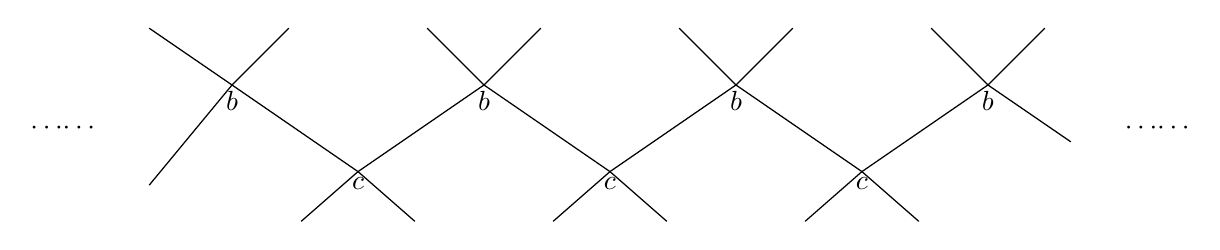
\begin{tikzpicture}[
  x=1cm,
  y=1cm,
  line cap=round,
  line join=round,
  every node/.style={inner sep=1pt}
]
  \coordinate (b1) at (2.8,0.55);
  \coordinate (c1) at (4.4,-0.55);
  \coordinate (b2) at (6.0,0.55);
  \coordinate (c2) at (7.6,-0.55);
  \coordinate (b3) at (9.2,0.55);
  \coordinate (c3) at (10.8,-0.55);
  \coordinate (b4) at (12.4,0.55);

  \draw[line width=.45pt]
    (1.75,1.27) -- (b1) -- (c1) -- (b2) -- (c2) --
    (b3) -- (c3) -- (b4) -- (13.45,-0.17);
  \draw[line width=.45pt] (1.75,-0.72) -- (b1) -- (3.52,1.27);
  \draw[line width=.45pt] (3.68,-1.18) -- (c1) -- (5.12,-1.18);
  \draw[line width=.45pt] (5.28,1.27) -- (b2) -- (6.72,1.27);
  \draw[line width=.45pt] (6.88,-1.18) -- (c2) -- (8.32,-1.18);
  \draw[line width=.45pt] (8.48,1.27) -- (b3) -- (9.92,1.27);
  \draw[line width=.45pt] (10.08,-1.18) -- (c3) -- (11.52,-1.18);
  \draw[line width=.45pt] (11.68,1.27) -- (b4) -- (13.12,1.27);

  \node[below=1pt] at (b1) {$b$};
  \node[below=1pt] at (b2) {$b$};
  \node[below=1pt] at (b3) {$b$};
  \node[below=1pt] at (b4) {$b$};
  \node[below=1pt] at (c1) {$c$};
  \node[below=1pt] at (c2) {$c$};
  \node[below=1pt] at (c3) {$c$};

  \node at (0.65,0) {$\cdots\!\cdots$};
  \node at (14.55,0) {$\cdots\!\cdots$};
\end{tikzpicture}

\end{center}
（注意：这是平展拓扑的主丛。）有一个同态
\[
  \varphi:\mathbb Z\longrightarrow\operatorname{GL}(2,\mathbb Z),
  \qquad
  \varphi(n)=
  \begin{pmatrix}
    1 & n\\
    0 & 1
  \end{pmatrix},
\]
借助它，可从 \(P\) 上的平凡环面 \(\mathbb G_m^2\) 及由 \(\varphi\) 导出的下降数据，
构造 \(S\) 上相对维数为 \(2\) 的环面 \(T\)。（注意：投影 \(P\to S\) 是平展拓扑的覆盖，
\emph{从而也}是 \((\mathbf{Sch})\) 的典范拓扑的覆盖；由于 \(\mathbb G_{m,P}^2\)
在 \(P\) 上仿射，上述下降数据必为有效的。）不难证明，\(T\) 在 \(a\) 的邻域中并非等平凡
\footnote{编者注：见下文 \SGARefLink{sga3:x:example:7-3}{7.3}。}（尽管它在 \(S-\{a\}\) 上平凡）。

将 \(S\) 取为具有两个不可约分量 \(S_1\) 和 \(S_2\)、它们相交于两点
\(a'\) 和 \(a''\) 的曲线，可得到此构造的一个变体。
这样能构造 \(S\) 上群为 \(\mathbb Z_S\) 的连通、局部平凡的主齐性丛 \(P\)，
进而得到一个局部平凡但非等平凡的伴随环面 \(T\)。

\SGARefTarget{sga3:x:section:2}\section*{2. 结构的无穷小变化}
\addcontentsline{toc}{section}{2. 结构的无穷小变化}

\footnote{编者注：为便于下文引用，添加了这一“回顾”。}
先回顾下列结果（\(S\) 局部 Noether 时，参见\ SGA~1，I，8.3；一般情形见
EGA~IV\textsubscript{4}，18.1.2）。

\medskip
\noindent\SGARefTarget{sga3:x:recall:2:0}\textbf{回顾 2.0。} ---
\textit{设 \(S\) 是预概形，\(S_0\) 是具有相同底集的子预概形。则函子
\[
  X\longmapsto X_0=X\times_S S_0
\]
是 \(S\) 上的平展预概形范畴与 \(S_0\) 上相应范畴之间的等价。}

\medskip
\noindent\SGARefTarget{sga3:x:proposition:2:1}%
\textbf{命题 2.1。} ---
\textit{设 \(S\) 是预概形，\(S_0\) 是具有相同底集的子预概形
（即由一个幂零元理想 \(\mathscr I\) 定义）。则函子
\[
  H\longmapsto H_0=H\times_S S_0
\]
从 \(S\) 上的乘法型群预概形范畴到 \(S_0\) 上相应范畴是全忠实的。}

\textit{此外，它在 \(S\) 上的拟等平凡乘法型群范畴与 \(S_0\) 上相应范畴之间诱导等价。}

先证明全忠实性，即若 \(H\) 和 \(G\) 是 \(S\) 上的乘法型群，则
\[
  \operatorname{Hom}_{S\text{-}\mathrm{gr}}(H,G)
  \longrightarrow
  \operatorname{Hom}_{S_0\text{-}\mathrm{gr}}(H_0,G_0)
\]
是双射。问题在 \(S\) 上是局部的，因此可以假定 \(S\) 仿射。
这时存在分裂 \(H\) 和 \(G\) 的忠实平坦拟紧态射 \(S'\to S\)。
令 \(S''=S'\times_S S'\)；分别以 \(H',G'\) 和 \(H'',G''\) 表示从
\(H,G\) 通过基变换 \(S'\to S\) 和 \(S''\to S\) 得到的群。
类似地定义 \(S'_0\) 和 \(S''_0\)；后者也同构于 \(S'_0\times_{S_0}S'_0\)。
得到一个行正合的交换图：
\begin{center}
  {\small
\begin{tikzcd}[column sep=2.1em, row sep=3.4em]
  \operatorname{Hom}_{S\text{-}\mathrm{gr.}}(H,G)
    \arrow[r]
    \arrow[d,"u"]
  &
  \operatorname{Hom}_{S'\text{-}\mathrm{gr.}}(H',G')
    \arrow[r,shift left=.65ex]
    \arrow[r,shift right=.65ex]
    \arrow[d,"u'"]
  &
  \operatorname{Hom}_{S''\text{-}\mathrm{gr.}}(H'',G'')
    \arrow[d,"u''"]
  \\
  \operatorname{Hom}_{S_0\text{-}\mathrm{gr.}}(H_0,G_0)
    \arrow[r]
  &
  \operatorname{Hom}_{S'_0\text{-}\mathrm{gr.}}(H'_0,G'_0)
    \arrow[r,shift left=.65ex]
    \arrow[r,shift right=.65ex]
  &
  \operatorname{Hom}_{S''_0\text{-}\mathrm{gr.}}(H''_0,G''_0),
\end{tikzcd}
}

\end{center}
因此，为证明 \(u\) 是双射，只需证明 \(u'\) 和 \(u''\) 是双射。
这将问题归约到 \(H\) 和 \(G\) 都可对角化的情形，因而它们形如 \(D_S(M)\) 和
\(D_S(N)\)，其中 \(M\) 和 \(N\) 是通常的交换群。类似地，
\[
  H_0=D_{S_0}(M),\qquad G_0=D_{S_0}(N).
\]
于是有交换图\footnote{编者注：通过交换右端的 \(M\) 和 \(N\)，已更正原文。}
\begin{center}
  {\small
\begin{tikzcd}[column sep=3.2em, row sep=3.5em]
  \operatorname{Hom}_{S\text{-}\mathrm{gr.}}(N_S,M_S)
    \arrow[r,"\sim"]
    \arrow[d]
  &
  \operatorname{Hom}_{S\text{-}\mathrm{gr.}}\!\bigl(D_S(M),D_S(N)\bigr)
    \arrow[d]
  \\
  \operatorname{Hom}_{S_0\text{-}\mathrm{gr.}}(N_{S_0},M_{S_0})
    \arrow[r,"\sim"]
  &
  \operatorname{Hom}_{S_0\text{-}\mathrm{gr.}}\!\bigl(D_{S_0}(M),D_{S_0}(N)\bigr),
\end{tikzcd}
}

\end{center}
其中水平箭头由 \SGARefLink{sga3:viii:corollary:1:4}{VIII~1.4} 为同构。
因此，只须证明同态
\begin{equation}
  \operatorname{Hom}_{S\text{-}\mathrm{gr}}(N_S,M_S)
  \longrightarrow
  \operatorname{Hom}_{S_0\text{-}\mathrm{gr}}(N_{S_0},M_{S_0})
  \tag{x}\label{sga3:x:proposition:2-1:equation:x}
\end{equation}
是双射；换言之，从 \(S\) 上的常交换群预概形到 \(S_0\) 上的常交换群预概形的函子
\(M_S\mapsto M_{S_0}\) 是全忠实的。现在，
\SGARefLink{sga3:x:proposition:2-1:equation:x}{(x)} 还等同于自然映射
\[
  \operatorname{Hom}_{\mathrm{gr}}(N,\Gamma(M_S))
  \longrightarrow
  \operatorname{Hom}_{\mathrm{gr}}(N,\Gamma(M_{S_0}))
\]
它由 \(\Gamma(M_S)\to\Gamma(M_{S_0})\) 导出。后一个映射显然是双射，
因为 \(\Gamma(M_S)\)，即从 \(S\) 到 \(M\) 的局部常值映射集，仅依赖于
\(S\) 的底拓扑空间。这就证明了所需断言。

为证明 \SGARefLink{sga3:x:proposition:2:1}{2.1} 的第二个断言，只须说明
\(S_0\) 上的每个拟等平凡乘法型群 \(H_0\) 都来自 \(S\) 上的一个拟等平凡乘法型群
\(H\)。设 \(S'_0\to S_0\) 是分裂 \(H_0\) 的平展满射态射。

由 \SGARefLink{sga3:x:recall:2:0}{2.0}，存在平展态射 \(S'\to S\) 及 \(S_0\)-同构
\[
  S'\times_S S_0\simeq S'_0.
\]
因此可以假定 \(S'_0\) 由 \(S'\) 通过约化得到。由于 \(H'_0\) 可对角化，
立即可见它同构于从 \(S'\) 上的可对角化群 \(H'\) 通过基变换 \(S'_0\to S'\)
得到的群。（注意：若 \(H'_0=D_{S'_0}(M)\)，取 \(H'=D_{S'}(M)\)。）照例令
\[
  S''=S'\times_S S',
  \qquad
  S'''=S'\times_S S'\times_S S',
\]
并类似地通过从 \(S\) 到 \(S_0\) 的基变换定义 \(S''_0\) 和 \(S'''_0\)。
它们也分别同构于 \(S'_0\) 在 \(S_0\) 上的纤维平方和纤维立方。
将已证明的全忠实性应用于 \((S'',S''_0)\) 和 \((S''',S'''_0)\)，可知
\(H'_0\) 关于 \(S'_0\to S_0\) 的自然下降数据（参见\ \SGARefLink{sga3:iv:definition:2:1}{IV~2.1}）
来自 \(H'\) 关于 \(S'\to S\) 的唯一确定的下降数据。
由于 \(H'\) 在 \(S'\) 上仿射，这个下降数据有效（SGA~1，VIII，
\SGARefLink{sga3:viii:proposition:2:1}{2.1}）。因此存在 \(S\)-群 \(H\)，使得
\[
  H\times_S S'=H'=D_{S'}(M),
\]
因而 \(H\) 是拟等平凡乘法型群。

再使用 \((S',S'_0)\) 的全忠实性，容易验证 \(H'_0\) 与 \(H'\times_{S'}S'_0\)
之间给定的同构来自 \(H_0\) 与 \(H\times_S S_0\) 之间的同构。
（这类结果的更形式化叙述，见 Giraud 正在撰写的关于下降理论的文章。%
\begingroup
\renewcommand{\thefootnote}{\(\ast\)}%
\footnote{参见\ J.~Giraud，“下降方法〔Méthode de la descente〕”， \emph{Bull.\
Soc.\ Math.\ France}, Mémoire~2 (1964).}%
\endgroup
\addtocounter{footnote}{-1})

\medskip
\noindent\SGARefTarget{sga3:x:corollary:2:2}%
\textbf{推论 2.2。} ---
\textit{设 \(H\) 是乘法型 \(S\)-群，令 \(H_0=H\times_S S_0\)。
则 \(H\) 是拟等平凡的（分别为局部等平凡、等平凡、局部平凡或平凡的），
当且仅当 \(H_0\) 具有相应性质。}

“仅当”方向是直接的。“当”方向在拟等平凡情形下已证明：由全忠实性，
只需知道 \(S_0\) 上的每个拟等平凡群都提升为 \(S\) 上的一个拟等平凡群。
同样的论证适用于“平凡”。对于“等平凡”，重复证明
\SGARefLink{sga3:x:proposition:2:1}{2.1} 第二个断言的论证，但取 \(S'_0\to S_0\)
为有限平展满射。局部等平凡与局部平凡的情形立即由等平凡与平凡的情形推出。

当 \(\mathscr I\) 幂零时，无须\emph{预先}假定 \(H\) 为乘法型，
即可略微推广 \SGARefLink{sga3:x:corollary:2:2}{2.2}。
\footnote{编者注：回顾，\SGARefLink{sga3:x:corollary:2:3}{2.3} 用于证明
定理~\SGARefLink{sga3:ix:theorem:3:6}{IX~3.6}~bis。}

\medskip
\noindent\SGARefTarget{sga3:x:corollary:2:3}%
\textbf{推论 2.3。} ---
\textit{假定定义 \(S_0\) 的理想 \(\mathscr I\) 局部幂零。
设 \(H\) 是 \(S\) 上的群预概形，并在 \(S\) 上平坦，令 \(H_0=H\times_S S_0\)。
则 \(H\) 是拟等平凡乘法型群，当且仅当 \(H_0\) 如此。}

假定 \(H_0\) 是拟等平凡乘法型群。证明 \(H\) 也如此。
问题对于平展拓扑是局部的，而由 \SGARefLink{sga3:x:recall:2:0}{2.0}，函子
\(S'\mapsto S'\times_S S_0\) 给出 \(S\) 上平展预概形范畴与 \(S_0\) 上
平展预概形范畴的等价。因此立即归约到 \(H_0\) 可对角化的情形，因而同构于
\(D_{S_0}(M)\)。令 \(G=D_S(M)\)。于是有同构
\[
  u_0:H_0\xrightarrow{\sim}G_0.
\]
我断言，\(u_0\) 来自唯一的同态 \(u:H\to G\)；它必为同构，因为
\(u_0\) 是同构，\(H\) 和 \(G\) 在 \(S\) 上平坦，且 \(\mathscr I\) 局部幂零。
\footnote{编者注：由于 \(u_0\) 是同构，只需证明对每个 \(h\in H\)，态射
\(\varphi:\mathscr O_{G,u(h)}\to\mathscr O_{H,h}\) 是双射。
它模 \(\mathscr I=\mathscr I_s\) 约化后为双射，其中 \(s\) 是 \(h\) 在
\(S\) 中的像；因此其余核 \(C\) 满足 \(C=\mathscr IC\)，而因 \(\mathscr I\)
幂零，得到 \(C=0\)。由于 \(\mathscr O_{H,h}\) 在 \(\mathscr O_{S,s}\) 上平坦，
\(\varphi\) 的核 \(K\) 同样满足 \(K=\mathscr IK\)，从而 \(K=0\)。}
这将证明 \SGARefLink{sga3:x:corollary:2:3}{2.3}。有（参见\ VIII~1~(xxx)）
\[
  \operatorname{Hom}_{S\text{-}\mathrm{gr}}(H,G)
  \simeq
  \operatorname{Hom}_{S\text{-}\mathrm{gr}}
  \bigl(M_S,
    \underline{\operatorname{Hom}}_{S\text{-}\mathrm{gr}}
      (H,\mathbb G_{m,S})\bigr),
\]
且右端还等同于
\[
  \operatorname{Hom}_{\mathrm{gr}}
  \bigl(M,
    \operatorname{Hom}_{S\text{-}\mathrm{gr}}
      (H,\mathbb G_{m,S})\bigr).
\]
因此，同态
\begin{equation}
  \operatorname{Hom}_{S\text{-}\mathrm{gr}}(H,G)
  \longrightarrow
  \operatorname{Hom}_{S_0\text{-}\mathrm{gr}}(H_0,G_0)
  \tag{x}\label{sga3:x:corollary:2-3:equation:x}
\end{equation}
同构于同态
\[
  \operatorname{Hom}_{\mathrm{gr}}
  \bigl(M,\operatorname{Hom}_{S\text{-}\mathrm{gr}}
    (H,\mathbb G_{m,S})\bigr)
  \longrightarrow
  \operatorname{Hom}_{\mathrm{gr}}
  \bigl(M,\operatorname{Hom}_{S_0\text{-}\mathrm{gr}}
    (H_0,\mathbb G_{m,S_0})\bigr)
\]
它由限制同态导出
\begin{equation}
  \operatorname{Hom}_{S\text{-}\mathrm{gr}}(H,\mathbb G_{m,S})
  \longrightarrow
  \operatorname{Hom}_{S_0\text{-}\mathrm{gr}}
    (H_0,\mathbb G_{m,S_0}).
  \tag{xx}\label{sga3:x:corollary:2-3:equation:xx}
\end{equation}
因此，只需证明 \SGARefLink{sga3:x:corollary:2-3:equation:xx}{(xx)} 是双射。
问题在 \(S\) 上是局部的，故可假定 \(S\) 仿射。由于 \(\mathbb G_{m,S}\)
交换且在 \(S\) 上平滑，可以应用 \SGARefLink{sga3:ix:theorem:3:6}{IX~3.6}，从而完成证明。

\medskip
\noindent\SGARefTarget{sga3:x:corollary:2:4}%
\textbf{推论 2.4。} ---
\textit{设 \(A\) 是剩余域为 \(k\) 的 Artin 局部环，
\(S=\operatorname{Spec}(A)\)，\(S_0=\operatorname{Spec}(k)\)。}\begin{enumerate}
\item[\SGAInlineRefTarget{sga3:x:corollary:2:4:item:i}(i)]\textit{\footnote{编者注：为突出非平凡的蕴含，陈述已改写为只保留这一方向。}
设 \(H\) 是平坦且局部有限型的 \(S\)-群预概形，使 \(H_0=H\times_S S_0\)
为乘法型。则 \(H\) 为乘法型、有限型且等平凡。
特别地，每个有限型乘法型 \(S\)-群预概形 \(H\) 都等平凡。}
\item[\SGAInlineRefTarget{sga3:x:corollary:2:4:item:ii}(ii)]\textit{函子 \(H\mapsto H_0\) 给出 \(A\) 上的有限型乘法型群范畴与
\(k\) 上相应范畴之间的等价。}
\end{enumerate}

事实上，设 \(H\) 如 \SGARefLink{sga3:x:corollary:2:4:item:i}{(i)} 所述。
则 \(H_0\) 为乘法型且局部有限型，因而有限型，所以由
\SGARefLink{sga3:x:proposition:1:4}{1.4} 是等平凡的。由
\SGARefLink{sga3:x:corollary:2:3}{2.3} 和 \SGARefLink{sga3:x:corollary:2:2}{2.2}，
\(H\) 因而为乘法型（从而有限型）且等平凡。断言
\SGARefLink{sga3:x:corollary:2:4:item:ii}{(ii)} 再由 \SGARefLink{sga3:x:proposition:2:1}{2.1} 得到。

\medskip
\noindent\SGARefTarget{sga3:x:corollary:2:5}%
\textbf{推论 2.5。} ---
\textit{设 \(S'\to S\) 是忠实平坦的纯不可分态射。}
\begin{enumerate}
\item[(i)]\textit{函子
\[
  H\longmapsto H'=H\times_S S'
\]
从 \(S\) 上乘法型群的范畴到 \(S'\) 上相应范畴是全忠实的。
此外，它在拟等平凡乘法型群的子范畴之间诱导等价。}
\item[(ii)]\textit{若 \(H\) 是乘法型群，则 \(H\) 是拟等平凡的
（分别为局部等平凡、等平凡、局部平凡或平凡的），当且仅当 \(H'\) 具有相应性质。}
\end{enumerate}

事实上，令
\[
  S''=S'\times_S S',
  \qquad
  S'''=S'\times_S S'\times_S S'.
\]
假设 \(S'\to S\) 是纯不可分态射，意味着对角浸入 \(S'\to S''\) 和
\(S'\to S'''\) 是满射，因此沿任一浸入的基变换都适用
\SGARefLink{sga3:x:proposition:2:1}{2.1} 和 \SGARefLink{sga3:x:corollary:2:2}{2.2}。
考虑到 \(S'\to S\) 对于预概形上的乘法型群的纤维范畴是有效下降态射
（因为它忠实平坦且拟紧\footnote{编者注：详细说明这一点 \ldots}），
断言由 \SGARefLink{sga3:x:proposition:2:1}{2.1} 和 \SGARefLink{sga3:x:corollary:2:2}{2.2}
形式地推出（形式化论证见前引 Giraud 的文章）。

\SGARefTarget{sga3:x:section:3}\section*{3. 结构的有限变化：完备基环}
\addcontentsline{toc}{section}{3. 结构的有限变化：完备基环}

\medskip
\noindent\SGARefTarget{sga3:x:lemma:3:1}\textbf{引理 3.1。} ---
\textit{设 \(A\) 是配备理想 \(I\) 的 Noether 环，且 \(A\) 对于 \(I\)-进拓扑
分离且完备；令 \(S=\operatorname{Spec}(A)\)，\(S_0=\operatorname{Spec}(A/I)\)。
设 \(G\) 和 \(H\) 是两个 \(S\)-群预概形，其中 \(G\) 为等平凡乘法型群，
\(H\) 在 \(S\) 上仿射，并且在 \(H_0=H\times_S S_0\) 的各点在 \(S\) 上平坦，
其中 \(H_0\) 为拟等平凡乘法型群。则自然映射
\[
  \operatorname{Hom}_{S\text{-}\mathrm{gr}}(G,H)
  \longrightarrow
  \operatorname{Hom}_{S_0\text{-}\mathrm{gr}}(G_0,H_0)
\]
是双射。}

对每个整数 \(n\geq 0\)，令
\[
  S_n=\operatorname{Spec}(A/I^{n+1}),
\]
并令 \(G_n,H_n\) 从 \(G,H\) 通过基变换 \(S_n\to S\) 得到。
由于 \(G/S\) 是等平凡乘法型群，且 \(H\) 在 \(S\) 上仿射，
\SGARefLink{sga3:ix:theorem:7:1}{IX~7.1} 表明自然同态
\[
  \operatorname{Hom}_{S\text{-}\mathrm{gr}}(G,H)
  \longrightarrow
  \varprojlim_n
  \operatorname{Hom}_{S_n\text{-}\mathrm{gr}}(G_n,H_n)
\]
是双射。另一方面，\SGARefLink{sga3:x:corollary:2:3}{2.3} 表明各 \(H_n\)
是拟等平凡乘法型群，而 \SGARefLink{sga3:x:proposition:2:1}{2.1} 表明逆系
\[
  \bigl(
    \operatorname{Hom}_{S_n\text{-}\mathrm{gr}}(G_n,H_n)
  \bigr)_n
\]
中的所有过渡同态都是同构。\SGARefLink{sga3:x:lemma:3:1}{引理~3.1} 立即得证。

\medskip
\noindent\SGARefTarget{sga3:x:theorem:3:2}%
\textbf{定理 3.2。} ---
\textit{设 \(A\) 是配备理想 \(I\) 的 Noether 环，且 \(A\) 对于 \(I\)-进拓扑
分离且完备，令 \(S=\operatorname{Spec}(A)\)，\(S_0=\operatorname{Spec}(A/I)\)。则：}
\begin{enumerate}
\item[\SGAInlineRefTarget{sga3:x:theorem:3:2:item:i}(i)]\textit{函子
\[
  H\longmapsto H_0=H\times_S S_0
\]
是 \(S\) 上的等平凡乘法型群范畴与 \(S_0\) 上相应范畴之间的等价。}
\item[\SGAInlineRefTarget{sga3:x:theorem:3:2:item:ii}(ii)]\textit{设 \(H\) 是 \(S\) 上的有限型乘法型群。
则 \(H\) 等平凡，当且仅当 \(H_0\) 等平凡。}
\end{enumerate}

\textit{证明。}
对于 \SGARefLink{sga3:x:theorem:3:2:item:i}{(i)}，可以重复
\SGARefLink{sga3:x:proposition:2:1}{2.1} 的证明，或使用
\SGARefLink{sga3:x:corollary:1:2}{1.2}。两种方法都用到如下事实：函子
\[
  S'\longmapsto S'_0=S'\times_S S_0
\]
从 \(S\) 上的有限平展概形范畴到 \(S_0\) 上的有限平展概形范畴是等价
（SGA~1，I，\SGARefLink{sga3:x:lemma:8-4}{8.4}）。等价地，归约到
\(S\) 连通（即 \(S_0\) 连通）的情形，并选定 \(S_0\) 的一个几何点 \(\xi\) 后，典范同态
\[
  \pi_1(S_0,\xi)\longrightarrow\pi_1(S,\xi)
\]
是同构。

下面证明 \SGARefLink{sga3:x:theorem:3:2:item:ii}{(ii)}，即若 \(H_0\) 等平凡，
则 \(H\) 等平凡。由 \SGARefLink{sga3:x:theorem:3:2:item:i}{(i)}，存在 \(S\) 上的
等平凡乘法型群 \(G\) 及 \(S_0\)-同构
\[
  u_0:G_0\xrightarrow{\sim}H_0.
\]
\footnote{编者注：下文扩充了原文。}
由于 \(H\) 有限型，\(H_0\) 和 \(G_0\) 也有限型。因此，由
\SGARefLink{sga3:ix:proposition:2:1}{IX~2.1}~b)，\(G\) 在 \(S\) 每一点处的型
都是有限生成阿贝尔群，从而 \(G\) 在 \(S\) 上有限型。此外，由
\SGARefLink{sga3:x:lemma:3:1}{3.1}，\(u_0\) 来自一个 \(S\)-群同态
\[
  u:G\longrightarrow H.
\]
最后，\(G\) 和 \(H\) 都是 \(S\) 上的有限型乘法型群，且 \(u_0\) 为同构。
由 \SGARefLink{sga3:ix:corollary:2:9}{IX~2.9} 可知 \(u\) 为同构，因为
\(S_0\) 在 \(S\) 中的每个邻域都等于 \(S\)。

\medskip
\noindent\SGARefTarget{sga3:x:corollary:3:3}%
\textbf{推论 3.3。} ---
\textit{设 \(A\) 是剩余域为 \(k\) 的完备 Noether 局部环。}
\begin{enumerate}
\item[\SGAInlineRefTarget{sga3:x:corollary:3:3:item:i}(i)]\textit{\(A\) 上的每个有限型乘法型群都是等平凡的。}
\item[(ii)]\textit{函子
\[
  H\longmapsto H\otimes_A k=H_0
\]
是 \(A\) 上与 \(k\) 上的有限型乘法型群范畴之间的等价。}
\end{enumerate}

\footnotemark[12]
首先，\SGARefLink{sga3:x:corollary:3:3:item:i}{(i)} 由
\SGARefLink{sga3:x:theorem:3:2}{3.2}~\SGARefLink{sga3:x:theorem:3:2:item:ii}{(ii)} 和
\SGARefLink{sga3:x:proposition:1:4}{1.4} 得到。其次，考虑到 \(H\) 有限型当且仅当
\(H_0\) 有限型（参见\ \SGARefLink{sga3:x:theorem:3:2}{3.2}~\SGARefLink{sga3:x:theorem:3:2:item:ii}{(ii)} 的证明），
\SGARefLink{sga3:x:theorem:3:2:item:ii}{(ii)} 由
\SGARefLink{sga3:x:theorem:3:2}{3.2}~\SGARefLink{sga3:x:theorem:3:2:item:i}{(i)} 得到。

\medskip
\noindent\SGARefTarget{sga3:x:remark:3:3:1}%
\textbf{注记 3.3.1。} ---
由 \SGARefLink{sga3:x:proposition:1:4}{1.4}，陈述
\SGARefLink{sga3:x:corollary:3:3}{3.3} 通过 \(k\) 的代数闭包 \(\Omega\) 的拓扑
Galois 群，给出了 \(A\) 上有限型乘法型群的完整分类。

\medskip
\noindent\SGARefTarget{sga3:x:remarks:3:4}%
\textbf{注记 3.4。} ---
在 \SGARefLink{sga3:x:theorem:3:2}{3.2} 的假设下（即 \(A\) 是 Noether 环，
对于 \(I\)-进拓扑分离且完备，而对 \(A/I\) 无其他假设），由第~5 目将可知函子
\[
  H\longmapsto H_0
\]
从 \(S\) 上有限型乘法型群范畴到 \(S_0\) 上相应范畴仍为全忠实的，
无须任何等平凡性假设。\footnote{编者注：明确此引用，或许在第~5 目中增添一个推论 \ldots}

然而，一般情况下它不是本质满射的。事实上，可能存在 \(S_0\) 上的有限型乘法型群
\(H_0\)，甚至可以是局部平凡的（但非等平凡），却不来自 \(S\) 上某个乘法型群
\(H\) 的约化。

为看出这一点，可取 \SGARefLink{sga3:x:paragraph:1:6}{1.6} 中非正规曲线上非等平凡乘法型群的任一例子。
显然可将曲线取为仿射曲线，记为 \(S_0\)，并嵌入仿射 \(2\)-空间；
因此它由 \(k[X,Y]\) 中的理想 \(J\) 定义。取 \(A\) 为 \(k[X,Y]\) 对于
\(J\)-进拓扑的完备化。则 \(A\) 是维数为 \(2\) 的正则环，\emph{从而}正规。
将在 \SGARefLink{sga3:x:theorem:5-16}{5.16} 中看到，\(S=\operatorname{Spec}(A)\)
上的每个有限型乘法型群因而都是等平凡的。所以，有限型且非等平凡的 \(H_0\)
不能来自 \(S\) 上的乘法型群 \(H\)，因为这样的 \(H\) 必然有限型，从而等平凡。

\medskip
\noindent\SGARefTarget{sga3:x:lemma:3:5}\textbf{引理 3.5。}%
\begingroup
\renewcommand{\thefootnote}{\(\ast\)}%
\footnote{关于这类问题的更系统论述，另参见\ \(\mathrm{VI}_{\mathrm B}\)，\SGARefLink{sga3:x:corollary:2:5}{2.5}。}%
\endgroup
\addtocounter{footnote}{-1}
---
\textit{设 \(S\) 是预概形，\(u:G\to H\) 是局部有限呈示且在 \(S\) 上平坦的
\(S\)-群预概形之间的同态。令 \(U\) 为使纤维上诱导的同态
\[
  u_s:G_s\longrightarrow H_s,
\]
平坦（分别为平滑、非分歧、平展或拟有限）的 \(s\in S\) 所成的集合。
则 \(U\) 是开集，且限制
\[
  u|_U:G|_U\longrightarrow H|_U
\]
平坦（分别为平滑、非分歧、平展或拟有限）。}

设 \(V\) 为 \(u\) 平坦（分别为 \(\ldots\)）的点集。
已知 \(V\) 开（局部 Noether 情形参见\ SGA~1，I 至 IV；一般情形见 EGA~IV
\footnote{编者注：明确这些引用。由于 \(G,H\) 局部有限呈示，\(u\) 局部有限呈示
（IV\textsubscript{1}，1.4.3~(v)）；对于平坦和拟有限，应用 IV\textsubscript{3}，
11.3.10 和 13.1.4；对于非分歧、平滑和平展，应用 IV\textsubscript{4}，17.4.1、
17.5.1 和 17.6.1；比较 \(\mathrm{VI}_{\mathrm B}\)，\SGARefLink{sga3:x:corollary:2:5}{2.5}。}），
且对位于 \(s\in S\) 上方的 \(x\in G\)，\(x\in V\) 当且仅当
\(u_s:G_s\to H_s\) 在 \(x\) 处平坦（分别为 \(\ldots\)）
（同一引用；对于平坦、平滑和平展，这里使用了 \(G\) 和 \(H\) 在 \(S\) 上的平坦性）。
由于 \(u_s\) 是局部代数群同态，这又等价于 \(u_s\) 处处平坦（分别为 \(\ldots\)）
（\(\mathrm{VI}_{\mathrm B}\)，\SGARefLink{sga3:x:remark:1:3}{1.3}），即 \(s\in U\)。
因此，\(U\) 是开集 \(V\) 在 \(G\) 的单位截面下的逆像，故为开集。
此外，\(V=G|_U\)，所以 \(G|_U\to H|_U\) 平坦（分别为 \(\ldots\)），证明完成。
（注意：在非分歧和拟有限情形中，无须对 \(G\) 和 \(H\) 作平坦性假设。）

\medskip
\noindent\SGARefTarget{sga3:x:lemma:3:6}\textbf{引理 3.6。} ---
\textit{设 \(H\) 是域 \(k\) 上的交换代数群，具有一个乘法型开子群 \(G\)。
则子概形族 \({}_nH\)，\(n>0\)，在 \(H\) 中概形稠密。
特别地，若对每个 \(n>0\) 有 \({}_nH={}_nG\)，则 \(H=G\)。}

这里 \({}_nH\) 表示 \(n\cdot\operatorname{id}_H\) 的核。\footnote{编者注：前句为新增。}
设 \(\bar{k}\) 是 \(k\) 的代数闭包。只须证明族 \(({}_nH_{\bar{k}})_{n>0}\)
在 \(H_{\bar{k}}\) 中概形稠密，因为这将推出 \(({}_nH)_{n>0}\) 在 \(H\) 中概形稠密
（参见\ \SGARefLink{sga3:ix:lemma:4:5}{IX~4.5}）。因此可以假定 \(k\) 代数闭，
从而 \(G=D_k(M)\)，其中 \(M\) 是通常的有限生成交换群。

令
\[
  M_0=M/\operatorname{Torsion}(M).
\]
则 \(T=D_k(M_0)\) 是 \(G\) 中最大的环面，且 \(H/T\) 有限。
所以 \(H(k)/T(k)\) 被某个整数 \(\nu>0\) 零化。
存在有限多个 \(g_i\in H(k)\)，使得
\[
  H=\coprod_i g_i\cdot G,
\]
且 \(g_i^\nu\in T(k)\)。由于 \(k\) 代数闭，映射
\(\nu\cdot\operatorname{id}_T\) 在
\[
  T(k)\simeq(k^\times)^d.
\]
上为满射。因此，将 \(g_i\) 换成 \(g_it_i^{-1}\)，其中 \(t_i\in T(k)\)
满足 \(t_i^\nu=g_i^\nu\)，可假定 \(g_i^\nu=1\)。若现在 \(n\) 是 \(\nu\) 的倍数，则
\[
  {}_nH\supset g_i\cdot{}_nG.
\]
当 \(n>0\) 变化时，由 \SGARefLink{sga3:ix:theorem:4:7}{IX~4.7}，族
\({}_nG\) 在 \(G\) 中概形稠密，故得 \SGARefLink{sga3:x:lemma:3:6}{3.6} 的结论。

\medskip
\noindent\SGARefTarget{sga3:x:theorem:3:7}%
\textbf{定理 3.7。} ---
\textit{设 \(A\) 是配备理想 \(I\) 的 Noether 环，且 \(A\) 对于 \(I\)-进拓扑
分离且完备；令 \(S=\operatorname{Spec}(A)\)，\(S_0=\operatorname{Spec}(A/I)\)。
设 \(H\) 是仿射有限型 \(S\)-群概形，在 \(H_0\) 的各点在 \(S\) 上平坦，
且 \(H_0=H\times_S S_0\) 为等平凡乘法型群。则 \(H\) 存在既开又闭的子群
\(G\)，它是等平凡乘法型（且有限型）的，并满足 \(G_0=H_0\)。}

由 \SGARefLink{sga3:x:theorem:3:2}{3.2}~\SGARefLink{sga3:x:theorem:3:2:item:i}{(i)}，
存在 \(S\) 上的等平凡乘法型群 \(G\) 及同构
\[
  u_0:G_0\xrightarrow{\sim}H_0.
\]
由 \SGARefLink{sga3:x:lemma:3:1}{3.1}，\(u_0\) 来自唯一的 \(S\)-群同态
\[
  u:G\longrightarrow H.
\]
使用 \SGARefLink{sga3:ix:corollary:6:6}{IX~6.6} 可知 \(u\) 是单态射：若
\(U\) 为使 \(u_s:G_s\to H_s\) 为单态射的 \(s\in S\) 所成的集合，
则 \(U\) 是 \(S_0\) 的开邻域，故等于 \(S\)，而 \(G|_U\to H|_U\) 为单态射。
由 \SGARefLink{sga3:ix:corollary:2:5}{IX~2.5}，\(u\) 甚至是闭浸入。

因此，\(G\) 在 \(S\) 上有限型，从而有限呈示。\footnote{编者注：前句为新增。}
将\SGARefLink{sga3:x:lemma:3:5}{引理~3.5} 应用于平展情形，存在 \(S_0\) 的开邻域
\(U\)，故 \(U=S\)，使 \(G|_U\to H|_U\) 平展。因此，\(u\) 平展，
又因它是平展单态射，故为开浸入。\footnote{编者注：参见\ EGA~IV\textsubscript{4}，17.9.1。}
证明完成。

\medskip
\noindent\SGARefTarget{sga3:x:corollary:3:8}%
\textbf{推论 3.8。} ---
\textit{设 \(A\) 是配备理想 \(I\) 的 Noether 环，且 \(A\) 对于 \(I\)-进拓扑
分离且完备；令 \(S=\operatorname{Spec}(A)\)，\(S_0=\operatorname{Spec}(A/I)\)。
设 \(H\) 是有限型 \(S\)-群预概形，在 \(S\) 上仿射且平坦。}

\textit{则 \(H\) 为等平凡乘法型群，当且仅当 \(H_0\) 如此，且 \(H\) 满足下面
\SGARefLink{sga3:x:corollary:3:8:item:a}{(a)} 和 \SGARefLink{sga3:x:corollary:3:8:item:b}{(b)}
中的任一条件；因而在前述假设下，这两个条件等价：}
\begin{enumerate}
\item[\SGAInlineRefTarget{sga3:x:corollary:3:8:item:a}(a)]\textit{\(H\) 的纤维为乘法型，
且其型在 \(S\) 的每个连通分量上恒定。}
\item[\SGAInlineRefTarget{sga3:x:corollary:3:8:item:b}(b)]\textit{\(H\) 交换，且各
\({}_nH\)，\(n>0\)，在 \(S\) 上有限。}
\end{enumerate}
\textit{下面的条件蕴含上述两个条件：}
\begin{enumerate}
\item[\SGAInlineRefTarget{sga3:x:corollary:3:8:item:c}(c)]\textit{\(H\) 的纤维连通。}
\end{enumerate}

当然，若 \(H\) 为乘法型（且等平凡），则由
\SGARefLink{sga3:ix:remark:1:4:1}{IX~1.4.1}~a) 和 \SGARefLink{sga3:x:proposition:2:1}{2.1}~c)，
\SGARefLink{sga3:x:corollary:3:8:item:a}{(a)} 和 \SGARefLink{sga3:x:corollary:3:8:item:b}{(b)} 成立。
因此只需证明“当”的方向。使用 \SGARefLink{sga3:x:theorem:3:7}{3.7} 给出的子群 \(G\)。
当 \SGARefLink{sga3:x:corollary:3:8:item:c}{(c)} 成立时，显然 \(G=H\)，无须再证。

在 \SGARefLink{sga3:x:corollary:3:8:item:b}{(b)} 的情形中，浸入 \(u:G\to H\) 诱导开浸入
\[
  {}_nu:{}_nG\longrightarrow{}_nH
\]
以及同构
\[
  ({}_nG)_0\xrightarrow{\sim}({}_nH)_0.
\]
由于 \({}_nH\) 在 \(S\) 上有限，立即得到 \({}_nu\) 为同构：其像的补集在
\(S\) 上有限，且约化为空集。由 \SGARefLink{sga3:x:lemma:3:6}{3.6}，纤维上的诱导态射
\[
  u_s:G_s\longrightarrow H_s
\]
都是同构。因此 \(u\) 满射，从而为同构。

最后，在 \SGARefLink{sga3:x:corollary:3:8:item:a}{(a)} 的情形中，可以假定 \(S\) 连通。
\footnote{编者注：原文说“即 \(S_0\) 连通”。由于 \(A\) 对于 \(I\)-进拓扑分离，
\(S_0\) 与 \(S\) 的每个连通分量相交；又由于 \(A\) 完备，\(S_0\) 与 \(S\)
的连通分量一一对应。}于是，对每个 \(s\in S\)，
\[
  u_s:G_s\longrightarrow H_s
\]
是 \(\kappa(s)\) 上相同型的乘法型代数群的单态射。
\footnote{编者注：这是因为对每个 \(s\in S_0\)，\(G_s\) 和 \(H_s\) 具有相同的型，
从而对每个 \(s\) 都如此。}这样的同态必为同构，从而再次完成证明。
\footnote{编者注：事实上，\(u\) 将再次为满射开浸入。}
扩张基域后，可以假定 \(\kappa(s)\) 上的两个群都可对角化。
断言于是由 \SGARefLink{sga3:viii:corollary:3:2}{VIII~3.2}~b) 以及如下事实得到：
同构的有限生成 \(\mathbb Z\)-模之间的满同态
\[
  M\longrightarrow N
\]
必为双射。

\medskip
\noindent\SGARefTarget{sga3:x:corollary:3:9}%
\textbf{推论 3.9。} ---
\textit{设 \(A\) 是配备理想 \(I\) 的 Noether 环，且 \(A\) 对于 \(I\)-进拓扑
分离且完备，令 \(S=\operatorname{Spec}(A)\)，设 \(H\) 是有限型 \(S\)-群预概形，
在 \(S\) 上仿射且平坦，并具有连通纤维。则 \(H\) 是等平凡环面，当且仅当
\(H_0=H\times_S\operatorname{Spec}(A/I)\) 是等平凡环面。}